\documentclass[1p]{elsarticle_modified}
%\bibliographystyle{elsarticle-num}

%\usepackage[colorlinks]{hyperref}
%\usepackage{abbrmath_seonhwa} %\Abb, \Ascr, \Acal ,\Abf, \Afrak
\usepackage{amsfonts}
\usepackage{amssymb}
\usepackage{amsmath}
\usepackage{amsthm}
\usepackage{scalefnt}
\usepackage{amsbsy}
\usepackage{kotex}
\usepackage{caption}
\usepackage{subfig}
\usepackage{color}
\usepackage{graphicx}
\usepackage{xcolor} %% white, black, red, green, blue, cyan, magenta, yellow
\usepackage{float}
\usepackage{setspace}
\usepackage{hyperref}

\usepackage{tikz}
\usetikzlibrary{arrows}

\usepackage{multirow}
\usepackage{array} % fixed length table
\usepackage{hhline}

%%%%%%%%%%%%%%%%%%%%%
\makeatletter
\renewcommand*\env@matrix[1][\arraystretch]{%
	\edef\arraystretch{#1}%
	\hskip -\arraycolsep
	\let\@ifnextchar\new@ifnextchar
	\array{*\c@MaxMatrixCols c}}
\makeatother %https://tex.stackexchange.com/questions/14071/how-can-i-increase-the-line-spacing-in-a-matrix
%%%%%%%%%%%%%%%

\usepackage[normalem]{ulem}

\newcommand{\msout}[1]{\ifmmode\text{\sout{\ensuremath{#1}}}\else\sout{#1}\fi}
%SOURCE: \msout is \stkout macro in https://tex.stackexchange.com/questions/20609/strikeout-in-math-mode

\newcommand{\cancel}[1]{
	\ifmmode
	{\color{red}\msout{#1}}
	\else
	{\color{red}\sout{#1}}
	\fi
}

\newcommand{\add}[1]{
	{\color{blue}\uwave{#1}}
}

\newcommand{\replace}[2]{
	\ifmmode
	{\color{red}\msout{#1}}{\color{blue}\uwave{#2}}
	\else
	{\color{red}\sout{#1}}{\color{blue}\uwave{#2}}
	\fi
}

\newcommand{\Sol}{\mathcal{S}} %segment
\newcommand{\D}{D} %diagram
\newcommand{\A}{\mathcal{A}} %arc


%%%%%%%%%%%%%%%%%%%%%%%%%%%%%5 test

\def\sl{\operatorname{\textup{SL}}(2,\Cbb)}
\def\psl{\operatorname{\textup{PSL}}(2,\Cbb)}
\def\quan{\mkern 1mu \triangleright \mkern 1mu}

\theoremstyle{definition}
\newtheorem{thm}{Theorem}[section]
\newtheorem{prop}[thm]{Proposition}
\newtheorem{lem}[thm]{Lemma}
\newtheorem{ques}[thm]{Question}
\newtheorem{cor}[thm]{Corollary}
\newtheorem{defn}[thm]{Definition}
\newtheorem{exam}[thm]{Example}
\newtheorem{rmk}[thm]{Remark}
\newtheorem{alg}[thm]{Algorithm}

\newcommand{\I}{\sqrt{-1}}
\begin{document}

%\begin{frontmatter}
%
%\title{Boundary parabolic representations of knots up to 8 crossings}
%
%%% Group authors per affiliation:
%\author{Yunhi Cho} 
%\address{Department of Mathematics, University of Seoul, Seoul, Korea}
%\ead{yhcho@uos.ac.kr}
%
%
%\author{Seonhwa Kim} %\fnref{s_kim}}
%\address{Center for Geometry and Physics, Institute for Basic Science, Pohang, 37673, Korea}
%\ead{ryeona17@ibs.re.kr}
%
%\author{Hyuk Kim}
%\address{Department of Mathematical Sciences, Seoul National University, Seoul 08826, Korea}
%\ead{hyukkim@snu.ac.kr}
%
%\author{Seokbeom Yoon}
%\address{Department of Mathematical Sciences, Seoul National University, Seoul, 08826,  Korea}
%\ead{sbyoon15@snu.ac.kr}
%
%\begin{abstract}
%We find all boundary parabolic representation of knots up to 8 crossings.
%
%\end{abstract}
%\begin{keyword}
%    \MSC[2010] 57M25 
%\end{keyword}
%
%\end{frontmatter}

%\linenumbers
%\tableofcontents
%
\newcommand\colored[1]{\textcolor{white}{\rule[-0.35ex]{0.8em}{1.4ex}}\kern-0.8em\color{red} #1}%
%\newcommand\colored[1]{\textcolor{white}{ #1}\kern-2.17ex	\textcolor{white}{ #1}\kern-1.81ex	\textcolor{white}{ #1}\kern-2.15ex\color{red}#1	}

{\Large $\underline{11a_{211}~(K11a_{211})}$}

\setlength{\tabcolsep}{10pt}
\renewcommand{\arraystretch}{1.6}
\vspace{1cm}\begin{tabular}{m{100pt}>{\centering\arraybackslash}m{274pt}}
\multirow{5}{120pt}{
	\centering
	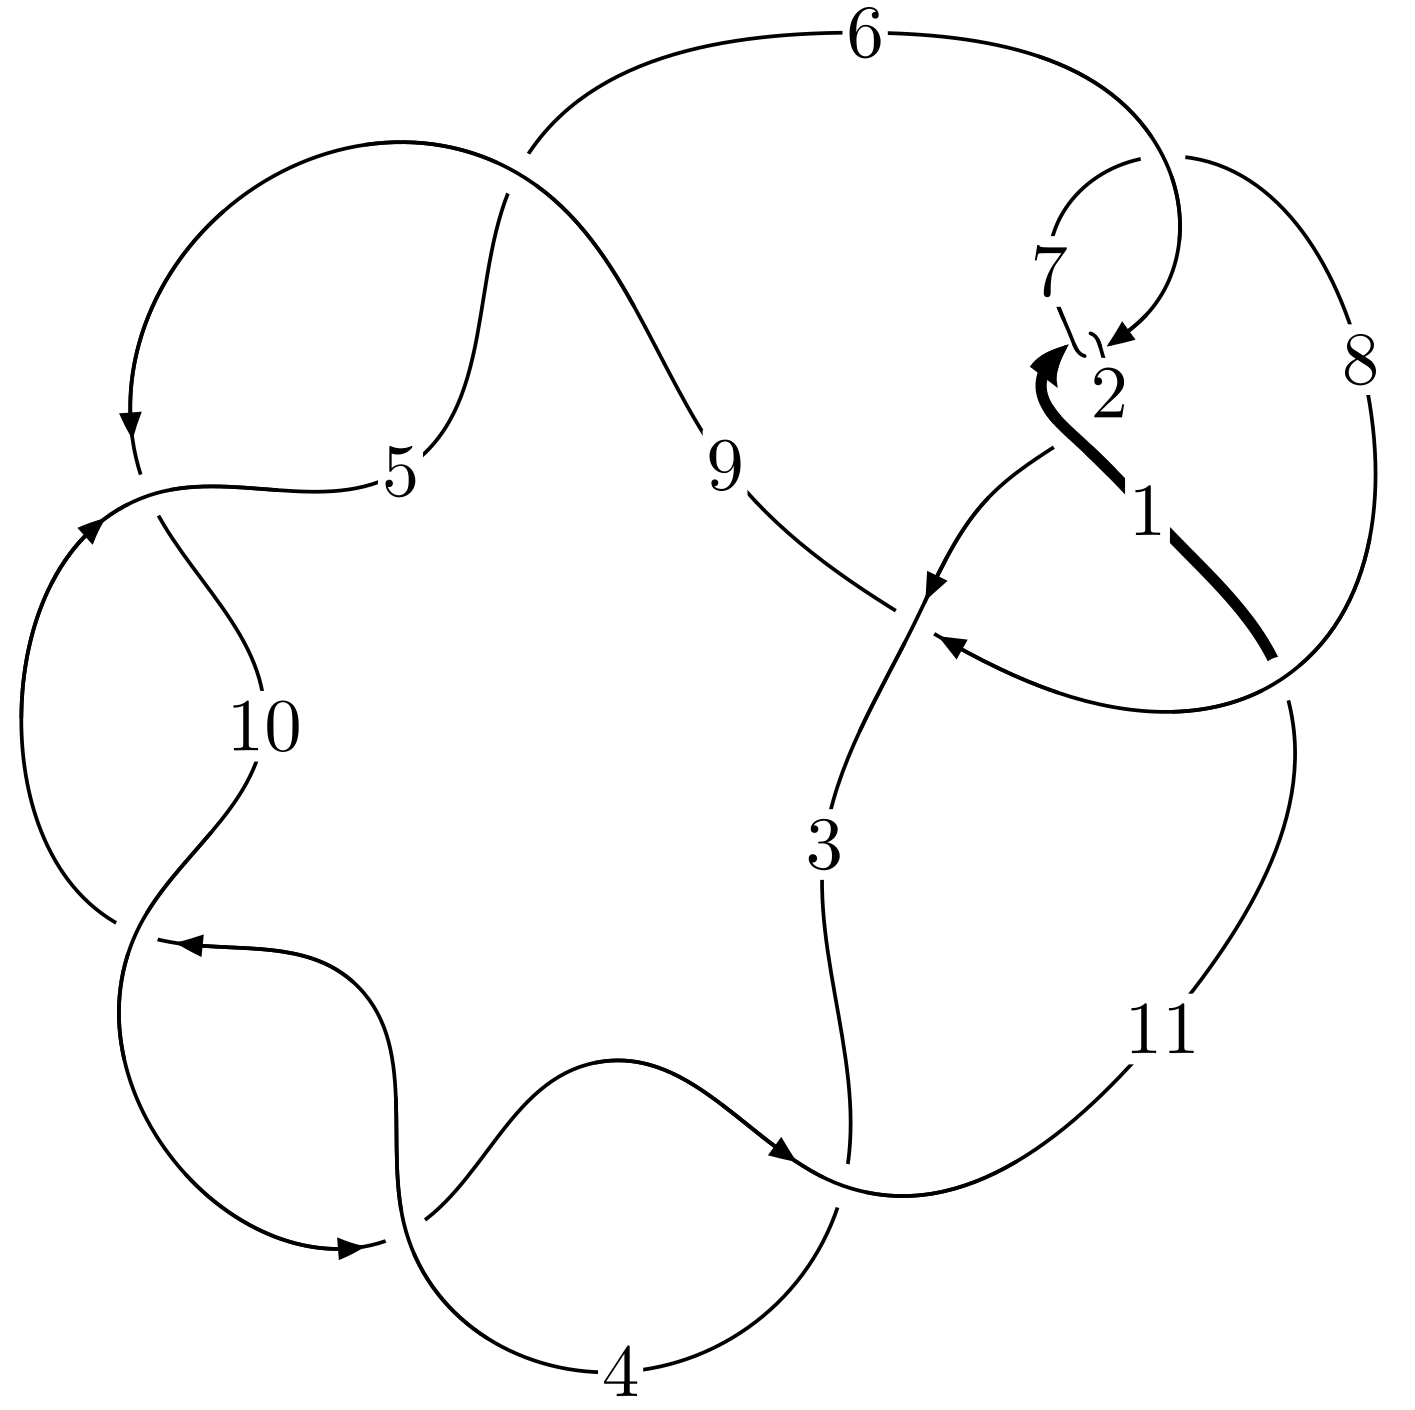
\includegraphics[width=112pt]{../../../GIT/diagram.site/Diagrams/png/460_11a_211.png}\\
\ \ \ A knot diagram\footnotemark}&
\allowdisplaybreaks
\textbf{Linearized knot diagam} \\
\cline{2-2}
 &
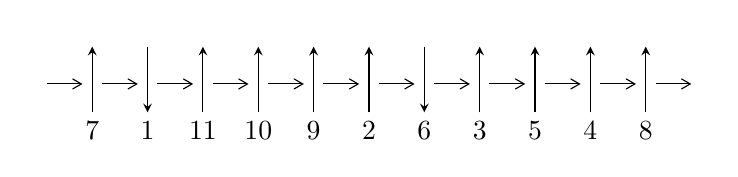
\begin{tikzpicture}[x=20pt, y=17pt]
	% nodes
	\node (C0) at (0, 0) {};
	\node (C1) at (1, 0) {};
	\node (C1U) at (1, +1) {};
	\node (C1D) at (1, -1) {7};

	\node (C2) at (2, 0) {};
	\node (C2U) at (2, +1) {};
	\node (C2D) at (2, -1) {1};

	\node (C3) at (3, 0) {};
	\node (C3U) at (3, +1) {};
	\node (C3D) at (3, -1) {11};

	\node (C4) at (4, 0) {};
	\node (C4U) at (4, +1) {};
	\node (C4D) at (4, -1) {10};

	\node (C5) at (5, 0) {};
	\node (C5U) at (5, +1) {};
	\node (C5D) at (5, -1) {9};

	\node (C6) at (6, 0) {};
	\node (C6U) at (6, +1) {};
	\node (C6D) at (6, -1) {2};

	\node (C7) at (7, 0) {};
	\node (C7U) at (7, +1) {};
	\node (C7D) at (7, -1) {6};

	\node (C8) at (8, 0) {};
	\node (C8U) at (8, +1) {};
	\node (C8D) at (8, -1) {3};

	\node (C9) at (9, 0) {};
	\node (C9U) at (9, +1) {};
	\node (C9D) at (9, -1) {5};

	\node (C10) at (10, 0) {};
	\node (C10U) at (10, +1) {};
	\node (C10D) at (10, -1) {4};

	\node (C11) at (11, 0) {};
	\node (C11U) at (11, +1) {};
	\node (C11D) at (11, -1) {8};
	\node (C12) at (12, 0) {};

	% arrows
	\draw[->,>={angle 60}]
	(C0) edge (C1) (C1) edge (C2) (C2) edge (C3) (C3) edge (C4) (C4) edge (C5) (C5) edge (C6) (C6) edge (C7) (C7) edge (C8) (C8) edge (C9) (C9) edge (C10) (C10) edge (C11) (C11) edge (C12) ;	\draw[->,>=stealth]
	(C1D) edge (C1U) (C2U) edge (C2D) (C3D) edge (C3U) (C4D) edge (C4U) (C5D) edge (C5U) (C6D) edge (C6U) (C7U) edge (C7D) (C8D) edge (C8U) (C9D) edge (C9U) (C10D) edge (C10U) (C11D) edge (C11U) ;
	\end{tikzpicture} \\
\hhline{~~} \\& 
\textbf{Solving Sequence} \\ \cline{2-2} 
 &
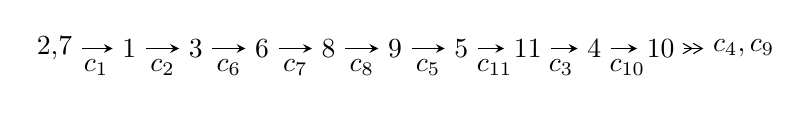
\begin{tikzpicture}[x=24pt, y=7pt]
	% node
	\node (A0) at (-1/8, 0) {2,7};
	\node (A1) at (1, 0) {1};
	\node (A2) at (2, 0) {3};
	\node (A3) at (3, 0) {6};
	\node (A4) at (4, 0) {8};
	\node (A5) at (5, 0) {9};
	\node (A6) at (6, 0) {5};
	\node (A7) at (7, 0) {11};
	\node (A8) at (8, 0) {4};
	\node (A9) at (9, 0) {10};
	\node (C1) at (1/2, -1) {$c_{1}$};
	\node (C2) at (3/2, -1) {$c_{2}$};
	\node (C3) at (5/2, -1) {$c_{6}$};
	\node (C4) at (7/2, -1) {$c_{7}$};
	\node (C5) at (9/2, -1) {$c_{8}$};
	\node (C6) at (11/2, -1) {$c_{5}$};
	\node (C7) at (13/2, -1) {$c_{11}$};
	\node (C8) at (15/2, -1) {$c_{3}$};
	\node (C9) at (17/2, -1) {$c_{10}$};
	\node (A10) at (41/4, 0) {$c_{4},c_{9}$};

	% edge
	\draw[->,>=stealth]	
	(A0) edge (A1) (A1) edge (A2) (A2) edge (A3) (A3) edge (A4) (A4) edge (A5) (A5) edge (A6) (A6) edge (A7) (A7) edge (A8) (A8) edge (A9) ;
	\draw[->>,>={angle 60}]	
	(A9) edge (A10);
\end{tikzpicture} \\ 

\end{tabular} \\

\footnotetext{
The image of knot diagram is generated by the software ``\textbf{Draw programme}" developed by Andrew Bartholomew(\url{http://www.layer8.co.uk/maths/draw/index.htm\#Running-draw}), where we modified some parts for our purpose(\url{https://github.com/CATsTAILs/LinksPainter}).
}\phantom \\ \newline 
\centering \textbf{Ideals for irreducible components\footnotemark of $X_{\text{par}}$} 
 
\begin{align*}
I^u_{1}&=\langle 
u^{33}+u^{32}+\cdots+u-1\rangle \\
\\
\end{align*}
\raggedright * 1 irreducible components of $\dim_{\mathbb{C}}=0$, with total 33 representations.\\
\footnotetext{All coefficients of polynomials are rational numbers. But the coefficients are sometimes approximated in decimal forms when there is not enough margin.}
\newpage
\renewcommand{\arraystretch}{1}
\centering \section*{I. $I^u_{1}= \langle u^{33}+u^{32}+\cdots+u-1 \rangle$}
\flushleft \textbf{(i) Arc colorings}\\
\begin{tabular}{m{7pt} m{180pt} m{7pt} m{180pt} }
\flushright $a_{2}=$&$\begin{pmatrix}1\\0\end{pmatrix}$ \\
\flushright $a_{7}=$&$\begin{pmatrix}0\\u\end{pmatrix}$ \\
\flushright $a_{1}=$&$\begin{pmatrix}1\\u^2\end{pmatrix}$ \\
\flushright $a_{3}=$&$\begin{pmatrix}u^2+1\\u^4\end{pmatrix}$ \\
\flushright $a_{6}=$&$\begin{pmatrix}- u\\u\end{pmatrix}$ \\
\flushright $a_{8}=$&$\begin{pmatrix}- u^3\\u^3+u\end{pmatrix}$ \\
\flushright $a_{9}=$&$\begin{pmatrix}u^9+2 u^7+3 u^5+2 u^3+u\\u^{11}+u^9+2 u^7+u^5+u^3+u\end{pmatrix}$ \\
\flushright $a_{5}=$&$\begin{pmatrix}- u^{21}-4 u^{19}+\cdots-2 u^3- u\\- u^{23}-3 u^{21}+\cdots-2 u^3+u\end{pmatrix}$ \\
\flushright $a_{11}=$&$\begin{pmatrix}- u^8- u^6- u^4+1\\u^8+2 u^6+2 u^4+2 u^2\end{pmatrix}$ \\
\flushright $a_{4}=$&$\begin{pmatrix}u^{20}+3 u^{18}+7 u^{16}+10 u^{14}+10 u^{12}+7 u^{10}+u^8-2 u^6-3 u^4- u^2+1\\- u^{20}-4 u^{18}-10 u^{16}-18 u^{14}-23 u^{12}-24 u^{10}-18 u^8-10 u^6-3 u^4\end{pmatrix}$ \\
\flushright $a_{10}=$&$\begin{pmatrix}- u^{32}-5 u^{30}+\cdots-2 u^2+1\\u^{32}+6 u^{30}+\cdots+2 u^4+2 u^2\end{pmatrix}$\\ \flushright $a_{10}=$&$\begin{pmatrix}- u^{32}-5 u^{30}+\cdots-2 u^2+1\\u^{32}+6 u^{30}+\cdots+2 u^4+2 u^2\end{pmatrix}$\\&\end{tabular}
\flushleft \textbf{(ii) Obstruction class $= -1$}\\~\\
\flushleft \textbf{(iii) Cusp Shapes $= 4 u^{31}+4 u^{30}+20 u^{29}+20 u^{28}+72 u^{27}+68 u^{26}+176 u^{25}+164 u^{24}+344 u^{23}+308 u^{22}+536 u^{21}+476 u^{20}+688 u^{19}+600 u^{18}+736 u^{17}+644 u^{16}+644 u^{15}+572 u^{14}+468 u^{13}+424 u^{12}+268 u^{11}+260 u^{10}+120 u^9+120 u^8+52 u^7+48 u^6+20 u^5+12 u^4+20 u^3+4 u^2+8 u+10$}\\~\\
\newpage\renewcommand{\arraystretch}{1}
\flushleft \textbf{(iv) u-Polynomials at the component}\newline \\
\begin{tabular}{m{50pt}|m{274pt}}
Crossings & \hspace{64pt}u-Polynomials at each crossing \\
\hline $$\begin{aligned}c_{1},c_{6}\end{aligned}$$&$\begin{aligned}
&u^{33}+u^{32}+\cdots+u-1
\end{aligned}$\\
\hline $$\begin{aligned}c_{2},c_{7}\end{aligned}$$&$\begin{aligned}
&u^{33}+11 u^{32}+\cdots+5 u-1
\end{aligned}$\\
\hline $$\begin{aligned}c_{3},c_{4},c_{5}\\c_{9},c_{10}\end{aligned}$$&$\begin{aligned}
&u^{33}+u^{32}+\cdots- u-1
\end{aligned}$\\
\hline $$\begin{aligned}c_{8}\end{aligned}$$&$\begin{aligned}
&u^{33}+u^{32}+\cdots+21 u-5
\end{aligned}$\\
\hline $$\begin{aligned}c_{11}\end{aligned}$$&$\begin{aligned}
&u^{33}-5 u^{32}+\cdots+33 u-7
\end{aligned}$\\
\hline
\end{tabular}\\~\\
\newpage\renewcommand{\arraystretch}{1}
\flushleft \textbf{(v) Riley Polynomials at the component}\newline \\
\begin{tabular}{m{50pt}|m{274pt}}
Crossings & \hspace{64pt}Riley Polynomials at each crossing \\
\hline $$\begin{aligned}c_{1},c_{6}\end{aligned}$$&$\begin{aligned}
&y^{33}+11 y^{32}+\cdots+5 y-1
\end{aligned}$\\
\hline $$\begin{aligned}c_{2},c_{7}\end{aligned}$$&$\begin{aligned}
&y^{33}+23 y^{32}+\cdots+41 y-1
\end{aligned}$\\
\hline $$\begin{aligned}c_{3},c_{4},c_{5}\\c_{9},c_{10}\end{aligned}$$&$\begin{aligned}
&y^{33}+43 y^{32}+\cdots+5 y-1
\end{aligned}$\\
\hline $$\begin{aligned}c_{8}\end{aligned}$$&$\begin{aligned}
&y^{33}+3 y^{32}+\cdots-299 y-25
\end{aligned}$\\
\hline $$\begin{aligned}c_{11}\end{aligned}$$&$\begin{aligned}
&y^{33}+7 y^{32}+\cdots-563 y-49
\end{aligned}$\\
\hline
\end{tabular}\\~\\
\newpage\flushleft \textbf{(vi) Complex Volumes and Cusp Shapes}
$$\begin{array}{c|c|c}  
\text{Solutions to }I^u_{1}& \I (\text{vol} + \sqrt{-1}CS) & \text{Cusp shape}\\
 \hline 
\begin{aligned}
u &= \phantom{-}0.783792 + 0.681225 I\end{aligned}
 & -0.01786 - 3.59856 I & \phantom{-}5.28807 + 3.52073 I \\ \hline\begin{aligned}
u &= \phantom{-}0.783792 - 0.681225 I\end{aligned}
 & -0.01786 + 3.59856 I & \phantom{-}5.28807 - 3.52073 I \\ \hline\begin{aligned}
u &= -0.101718 + 1.035980 I\end{aligned}
 & -6.05867 - 3.57865 I & -2.55817 + 4.87055 I \\ \hline\begin{aligned}
u &= -0.101718 - 1.035980 I\end{aligned}
 & -6.05867 + 3.57865 I & -2.55817 - 4.87055 I \\ \hline\begin{aligned}
u &= -0.812759 + 0.656775 I\end{aligned}
 & -9.39854 + 5.15635 I & \phantom{-}4.07009 - 1.99825 I \\ \hline\begin{aligned}
u &= -0.812759 - 0.656775 I\end{aligned}
 & -9.39854 - 5.15635 I & \phantom{-}4.07009 + 1.99825 I \\ \hline\begin{aligned}
u &= \phantom{-}0.064287 + 0.949488 I\end{aligned}
 & -2.15241 + 1.32489 I & \phantom{-}2.26975 - 5.19264 I \\ \hline\begin{aligned}
u &= \phantom{-}0.064287 - 0.949488 I\end{aligned}
 & -2.15241 - 1.32489 I & \phantom{-}2.26975 + 5.19264 I \\ \hline\begin{aligned}
u &= -0.755741 + 0.727580 I\end{aligned}
 & \phantom{-}3.31791 + 0.71142 I & \phantom{-}11.21363 - 1.67863 I \\ \hline\begin{aligned}
u &= -0.755741 - 0.727580 I\end{aligned}
 & \phantom{-}3.31791 - 0.71142 I & \phantom{-}11.21363 + 1.67863 I \\ \hline\begin{aligned}
u &= \phantom{-}0.721580 + 0.791474 I\end{aligned}
 & \phantom{-}1.87533 + 2.23676 I & \phantom{-}7.14983 - 4.95590 I \\ \hline\begin{aligned}
u &= \phantom{-}0.721580 - 0.791474 I\end{aligned}
 & \phantom{-}1.87533 - 2.23676 I & \phantom{-}7.14983 + 4.95590 I \\ \hline\begin{aligned}
u &= \phantom{-}0.113164 + 1.080920 I\end{aligned}
 & -15.7697 + 4.7978 I & -2.88521 - 3.43471 I \\ \hline\begin{aligned}
u &= \phantom{-}0.113164 - 1.080920 I\end{aligned}
 & -15.7697 - 4.7978 I & -2.88521 + 3.43471 I \\ \hline\begin{aligned}
u &= -0.564868 + 0.931483 I\end{aligned}
 & -3.48793 - 2.09474 I & \phantom{-}0.20074 + 2.52182 I \\ \hline\begin{aligned}
u &= -0.564868 - 0.931483 I\end{aligned}
 & -3.48793 + 2.09474 I & \phantom{-}0.20074 - 2.52182 I \\ \hline\begin{aligned}
u &= \phantom{-}0.529302 + 0.992831 I\end{aligned}
 & -13.31430 + 1.59055 I & -0.39166 - 2.82040 I \\ \hline\begin{aligned}
u &= \phantom{-}0.529302 - 0.992831 I\end{aligned}
 & -13.31430 - 1.59055 I & -0.39166 + 2.82040 I \\ \hline\begin{aligned}
u &= -0.767004 + 0.867736 I\end{aligned}
 & -5.87675 - 2.88651 I & \phantom{-}5.60693 + 2.86051 I \\ \hline\begin{aligned}
u &= -0.767004 - 0.867736 I\end{aligned}
 & -5.87675 + 2.88651 I & \phantom{-}5.60693 - 2.86051 I \\ \hline\begin{aligned}
u &= \phantom{-}0.689725 + 0.931969 I\end{aligned}
 & \phantom{-}1.43951 + 3.16744 I & \phantom{-}6.20217 - 0.82428 I \\ \hline\begin{aligned}
u &= \phantom{-}0.689725 - 0.931969 I\end{aligned}
 & \phantom{-}1.43951 - 3.16744 I & \phantom{-}6.20217 + 0.82428 I \\ \hline\begin{aligned}
u &= -0.704961 + 0.976337 I\end{aligned}
 & \phantom{-}2.56175 - 6.26830 I & \phantom{-}9.09411 + 7.22384 I \\ \hline\begin{aligned}
u &= -0.704961 - 0.976337 I\end{aligned}
 & \phantom{-}2.56175 + 6.26830 I & \phantom{-}9.09411 - 7.22384 I \\ \hline\begin{aligned}
u &= \phantom{-}0.706642 + 1.006440 I\end{aligned}
 & -0.99856 + 9.23572 I & \phantom{-}3.44794 - 8.32004 I \\ \hline\begin{aligned}
u &= \phantom{-}0.706642 - 1.006440 I\end{aligned}
 & -0.99856 - 9.23572 I & \phantom{-}3.44794 + 8.32004 I \\ \hline\begin{aligned}
u &= -0.710292 + 1.026450 I\end{aligned}
 & -10.5163 - 10.8805 I & \phantom{-}2.22808 + 6.70699 I \\ \hline\begin{aligned}
u &= -0.710292 - 1.026450 I\end{aligned}
 & -10.5163 + 10.8805 I & \phantom{-}2.22808 - 6.70699 I \\ \hline\begin{aligned}
u &= \phantom{-}0.648089 + 0.272678 I\end{aligned}
 & -11.39430 + 2.64374 I & \phantom{-}3.80222 - 2.50255 I \\ \hline\begin{aligned}
u &= \phantom{-}0.648089 - 0.272678 I\end{aligned}
 & -11.39430 - 2.64374 I & \phantom{-}3.80222 + 2.50255 I\\
 \hline 
 \end{array}$$\newpage$$\begin{array}{c|c|c}  
\text{Solutions to }I^u_{1}& \I (\text{vol} + \sqrt{-1}CS) & \text{Cusp shape}\\
 \hline 
\begin{aligned}
u &= -0.526368 + 0.248614 I\end{aligned}
 & -2.09314 - 1.78280 I & \phantom{-}4.63198 + 4.39540 I \\ \hline\begin{aligned}
u &= -0.526368 - 0.248614 I\end{aligned}
 & -2.09314 + 1.78280 I & \phantom{-}4.63198 - 4.39540 I \\ \hline\begin{aligned}
u &= \phantom{-}0.374260\phantom{ +0.000000I}\end{aligned}
 & \phantom{-}0.658769\phantom{ +0.000000I} & \phantom{-}15.2590\phantom{ +0.000000I}\\
 \hline 
 \end{array}$$\newpage
\newpage\renewcommand{\arraystretch}{1}
\centering \section*{ II. u-Polynomials}
\begin{tabular}{m{50pt}|m{274pt}}
Crossings & \hspace{64pt}u-Polynomials at each crossing \\
\hline $$\begin{aligned}c_{1},c_{6}\end{aligned}$$&$\begin{aligned}
&u^{33}+u^{32}+\cdots+u-1
\end{aligned}$\\
\hline $$\begin{aligned}c_{2},c_{7}\end{aligned}$$&$\begin{aligned}
&u^{33}+11 u^{32}+\cdots+5 u-1
\end{aligned}$\\
\hline $$\begin{aligned}c_{3},c_{4},c_{5}\\c_{9},c_{10}\end{aligned}$$&$\begin{aligned}
&u^{33}+u^{32}+\cdots- u-1
\end{aligned}$\\
\hline $$\begin{aligned}c_{8}\end{aligned}$$&$\begin{aligned}
&u^{33}+u^{32}+\cdots+21 u-5
\end{aligned}$\\
\hline $$\begin{aligned}c_{11}\end{aligned}$$&$\begin{aligned}
&u^{33}-5 u^{32}+\cdots+33 u-7
\end{aligned}$\\
\hline
\end{tabular}\newpage\renewcommand{\arraystretch}{1}
\centering \section*{ III. Riley Polynomials}
\begin{tabular}{m{50pt}|m{274pt}}
Crossings & \hspace{64pt}Riley Polynomials at each crossing \\
\hline $$\begin{aligned}c_{1},c_{6}\end{aligned}$$&$\begin{aligned}
&y^{33}+11 y^{32}+\cdots+5 y-1
\end{aligned}$\\
\hline $$\begin{aligned}c_{2},c_{7}\end{aligned}$$&$\begin{aligned}
&y^{33}+23 y^{32}+\cdots+41 y-1
\end{aligned}$\\
\hline $$\begin{aligned}c_{3},c_{4},c_{5}\\c_{9},c_{10}\end{aligned}$$&$\begin{aligned}
&y^{33}+43 y^{32}+\cdots+5 y-1
\end{aligned}$\\
\hline $$\begin{aligned}c_{8}\end{aligned}$$&$\begin{aligned}
&y^{33}+3 y^{32}+\cdots-299 y-25
\end{aligned}$\\
\hline $$\begin{aligned}c_{11}\end{aligned}$$&$\begin{aligned}
&y^{33}+7 y^{32}+\cdots-563 y-49
\end{aligned}$\\
\hline
\end{tabular}
\vskip 2pc
\end{document}